\section{Recurrent Neural Networks}
\subsection{Processing Sequences}
So far, all the deep neural networks that we studied (MLPs, CNNs) had the same \emph{feed-forward} global structure: the network receives an input of fixed size, which is fed into the successive layers of the network, which produces a fixed-size output. This is known as a \emph{one-to-one} model, and is mostly used for image classification.

When considering other applications, we would like more flexibility on the input and output sizes. For image captioning, we would like a \emph{one-to-many} model, where the input is a fixed size image, and the output a sentence of variable length. For text classification, such as sentiment analysis, we would like a \emph{many-to-one} model, where the input is a sentence of variable length and the output a fixed-size vector of class probabilities. Finally, we might want both the input and output to be variable in length, for instance in the case of machine translation: this requires a \emph{many-to-many} model.

\begin{figure}[H]
    \centering
    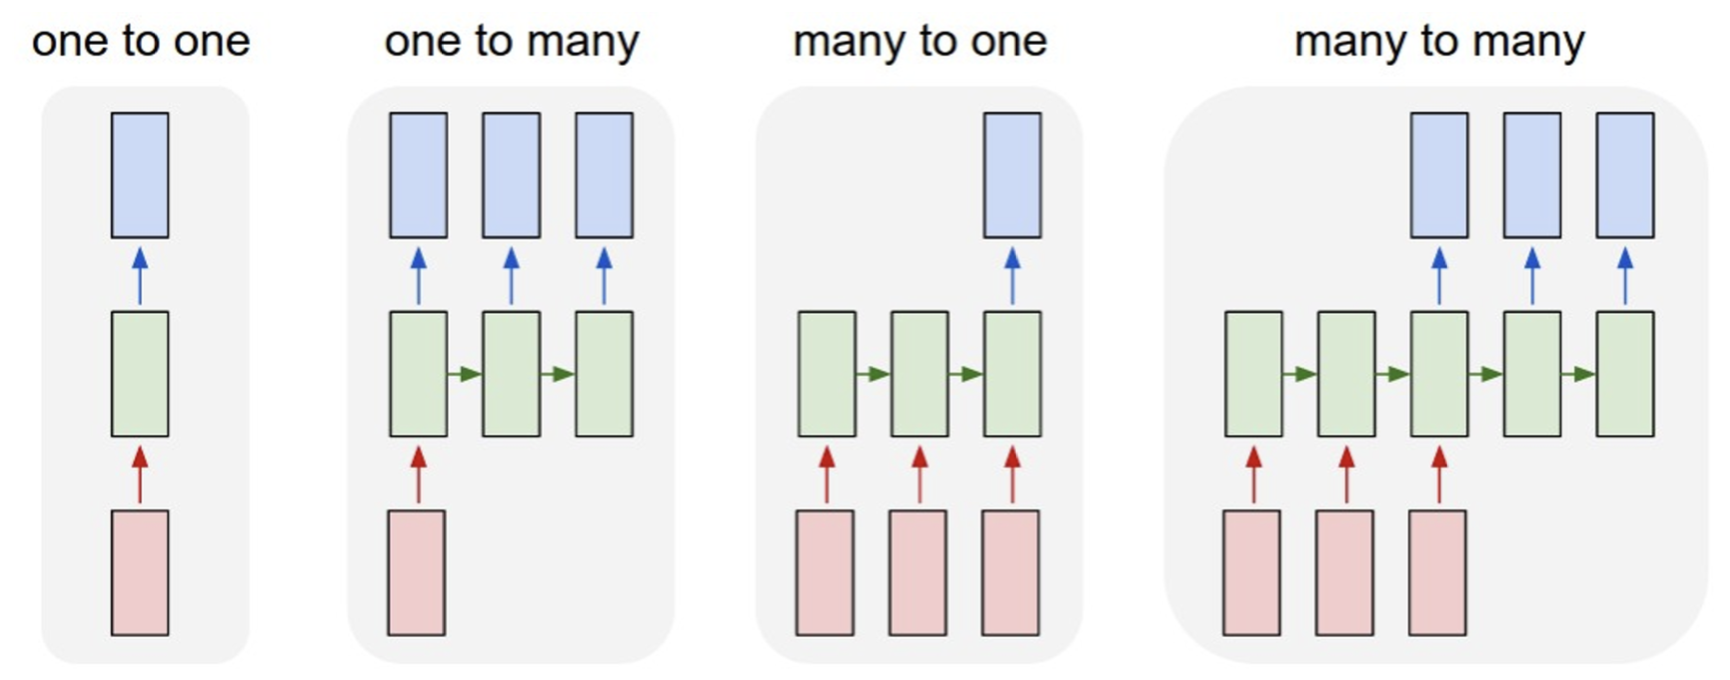
\includegraphics[width=.8\textwidth]{rnn/sequences.png}
\end{figure}

\emph{Recurrent Neural Networks} (RNNs) is a general paradigm which allows to handle all these different setups.

\subsection{Simple Recurrent Neural Network}
\subsubsection{General form}
\begin{wrapfigure}{r}{0.2\textwidth}
    \centering
    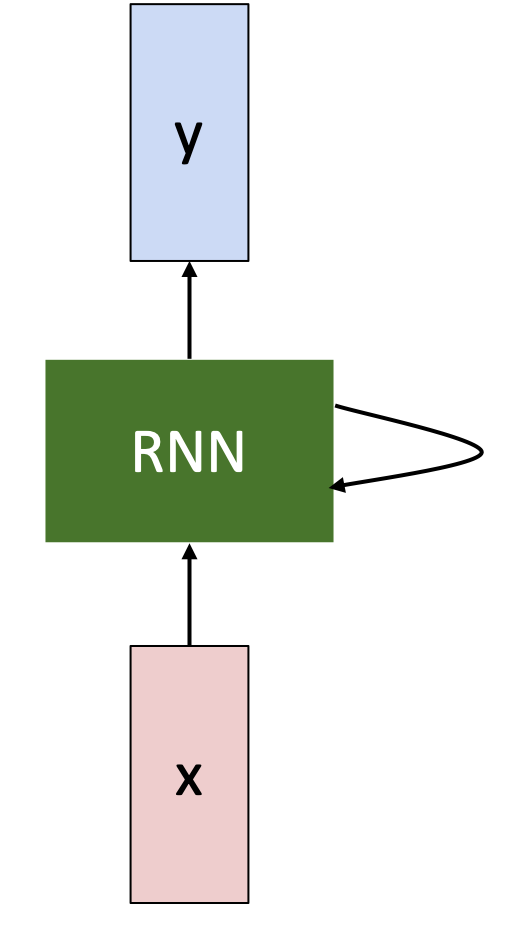
\includegraphics[width=.2\textwidth]{rnn/vanilla-rnn.png}
    \caption{A simple RNN.}
\end{wrapfigure}
In its simplest form, a Recurrent Neural Network possesses an internal hidden state which is updated each time that it reads an input. The handling of a sequential input (for instance, a sentence) follows this update loop: a fixed-size bit of the input is fed into the network, and is combined with the internal hidden state to produce an output and update the state. The next bit of the input is then fed to the network, and so on.

Formally, this can be written as a recurrence relationship:
\begin{equation*}
    h_t = f_W(h_{t-1}, x_t)
\end{equation*}
where $x$ is a sequence of vectors, $(h_t)_t$ is the sequence of hidden states, and $f_W$ is our network depending on some parameter $W$. To produce an output at each time step, we can simply transform the hidden state into an output using a feed-forward neural network:
\begin{equation*}
    y_t = g_{W'}(h_t)
\end{equation*}
Note that the same functions $f, g$ and the same parameters $W, W'$ are used at each step, only the internal state changes.

\subsubsection{A vanilla RNN}
We can create a simple RNN built around a single hidden vector $h_t$:
\begin{equation*}
    \begin{aligned}
        h_t &= \tanh\left(W_h h_{t-1} + W_x x_t\right)\\
        y_t &= W_y h_t
    \end{aligned}
\end{equation*}

\subsubsection{Computational graphs of RNNs}
Alongside with this intuition of RNNs as networks with hidden cells, it is also useful to think of RNNs as computational graphs. The graph of an RNN can be unfolded over multiple time steps, making explicit the inputs and gradient flow.
\begin{figure}[H]
    \centering
    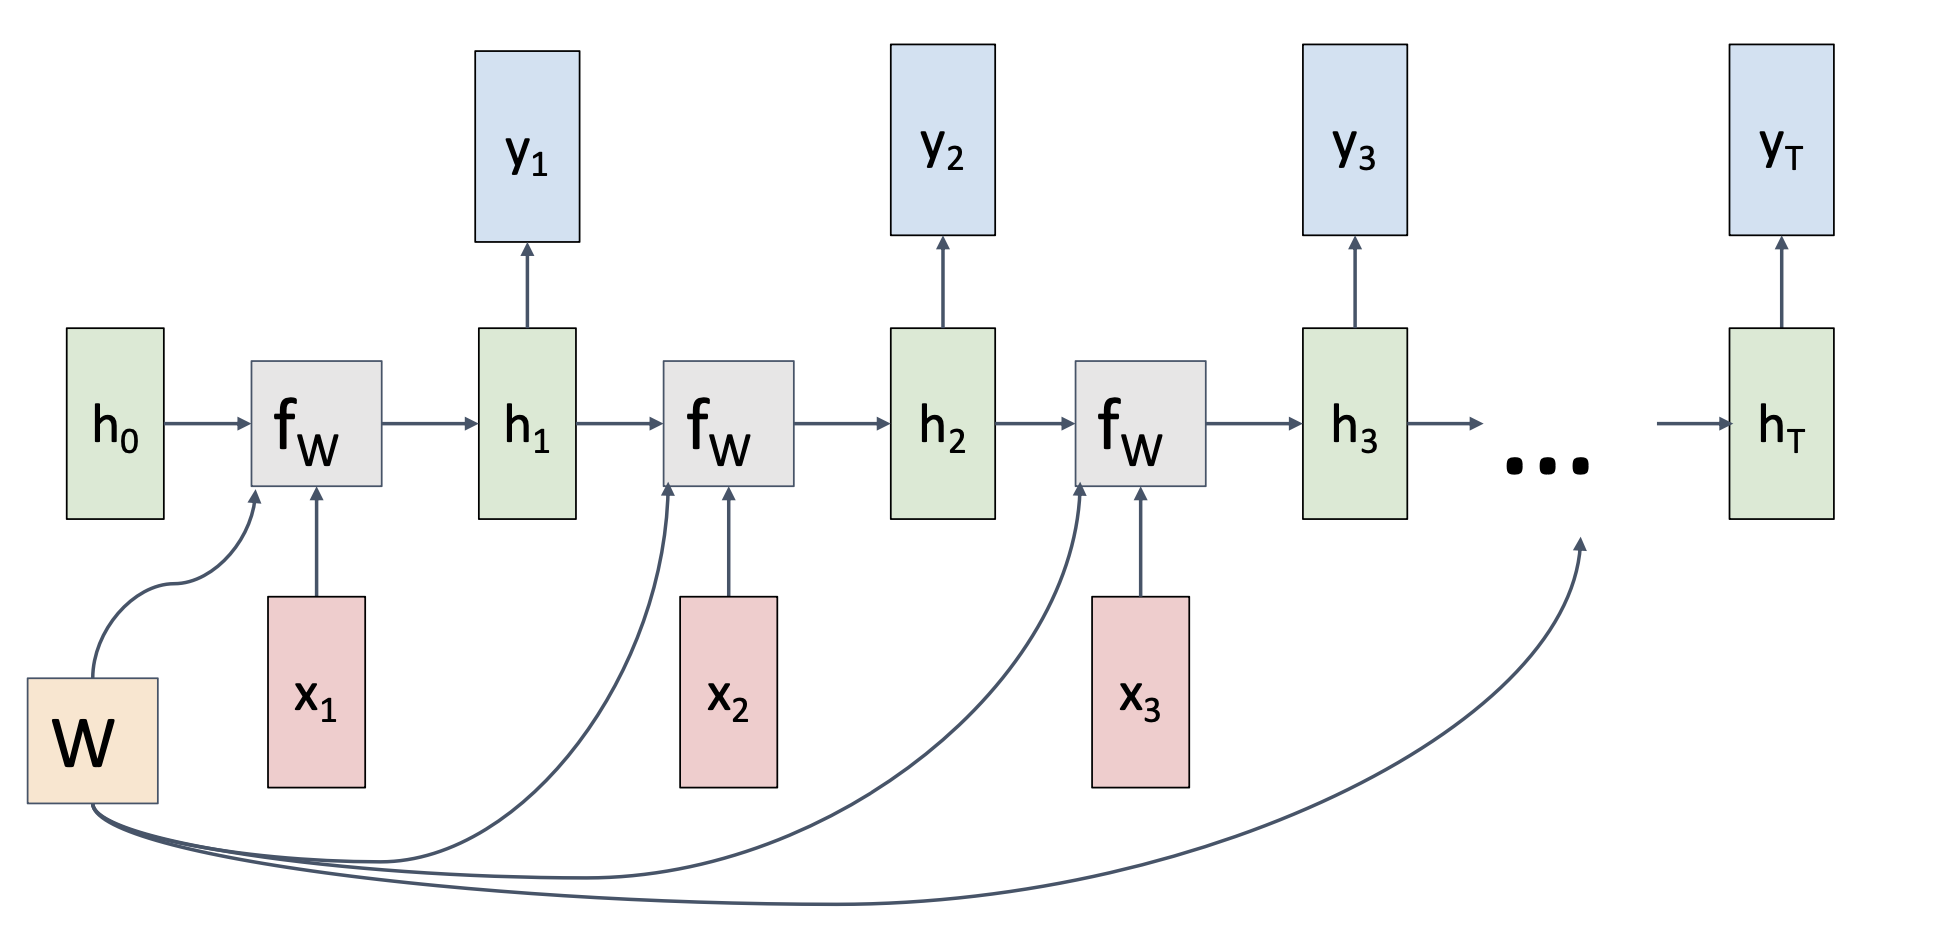
\includegraphics[width=.7\textwidth]{rnn/rnn-graph.png}
    \caption{Unfolded computational graph of an RNN.}
\end{figure}
The initial hidden state $h_0$ is often initialized to 0 in most contexts. It is then fed to the $f_W$ function with the first input $x_1$, which produces the new hidden state $h_1$. This hidden state can be used to compute the output $y_1$.

Note that the parameter $W$ remains the same for all; when computing the gradient $\frac{\partial\L}{\partial W}$, we will sum all the gradients coming from each time step to compute the total gradient.

This unfolded view also allows to understand the relationship with the loss more explicitly.
\begin{figure}[H]
    \centering
    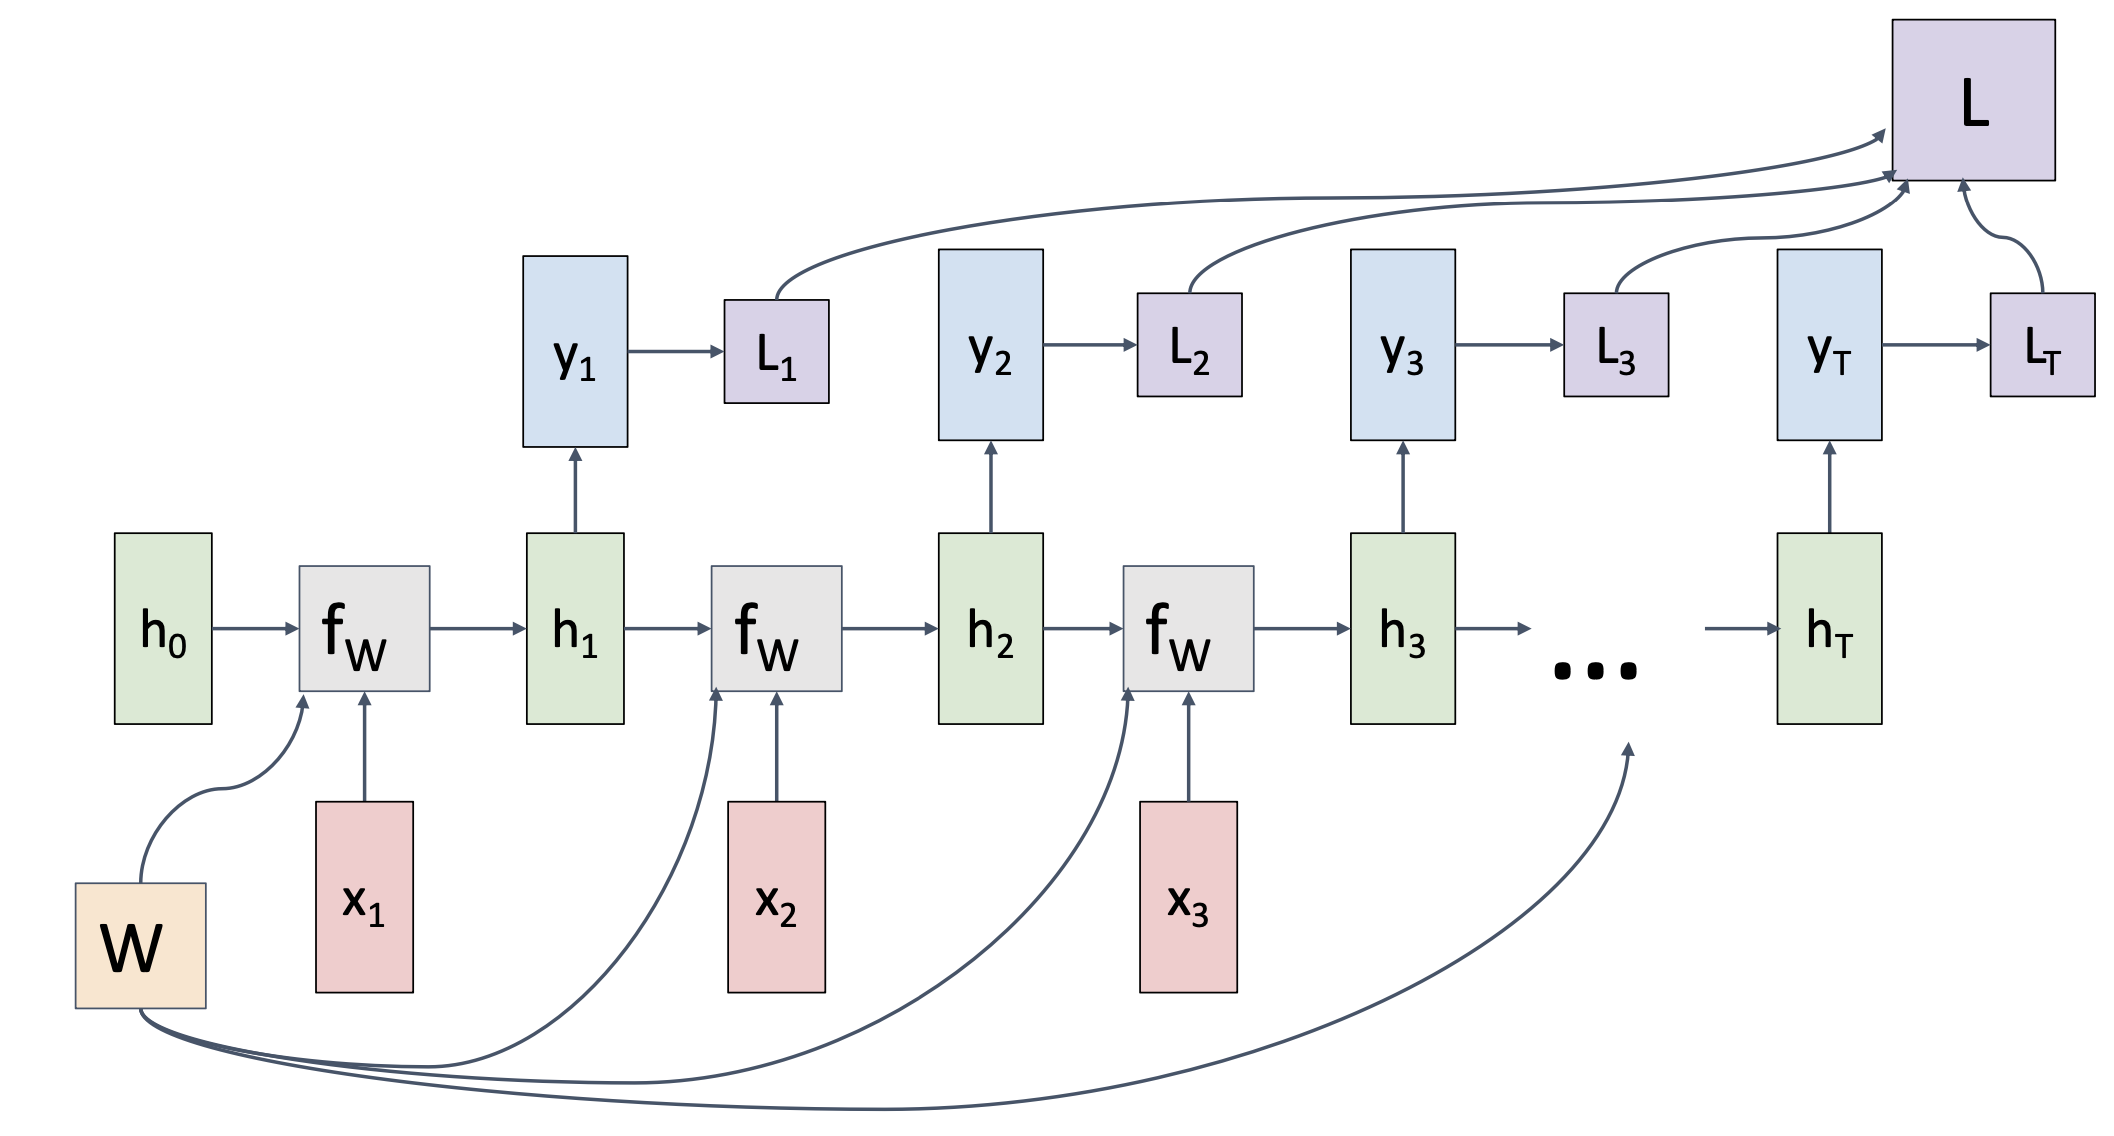
\includegraphics[width=.7\textwidth]{rnn/graph-loss.png}
    \caption{Loss of the unfolded graph.}
\end{figure}
Each output $y_t$ produced can be fed into some loss, for instance by comparing it to some ground truth label. The individual losses $\L_t$ can then be summed into a total loss $\L$, from which the backpropagation will start. Therefore, if we want to compute the gradient $\frac{\partial\L}{\partial W}$, the gradient flow will start in $\L$, separate itself into the different temporal steps $\L_t$, and then combine itself back to $W$ since the parameter is the same at each time step. This is called \emph{backpropagation through time}, as the forward pass is done by generating outputs at increasing time steps, while the backward pass is done starting from the most recently generated outputs.

\subsubsection{Many-to-one, one-to-many, many-to-many}
The previous examples involve a mechanism in which an output $y_t$ is produced for each input $x_t$. In the case of other types of models (many-to-one, one-to-many, many-to-many), we might produce no output for certain inputs, or outputs without inputs.

\paragraph*{Many-to-one}
In the many-to-one situation, we usually decide to produce an output only for the final input. The decision is therefore made based only on the final hidden state of the layer, $h_T$; the intuition behind this is that $h_T$ depends on all the previous hidden states $h_t$, and is therefore able to store the information used for the final decision.
\begin{figure}[H]
    \centering
    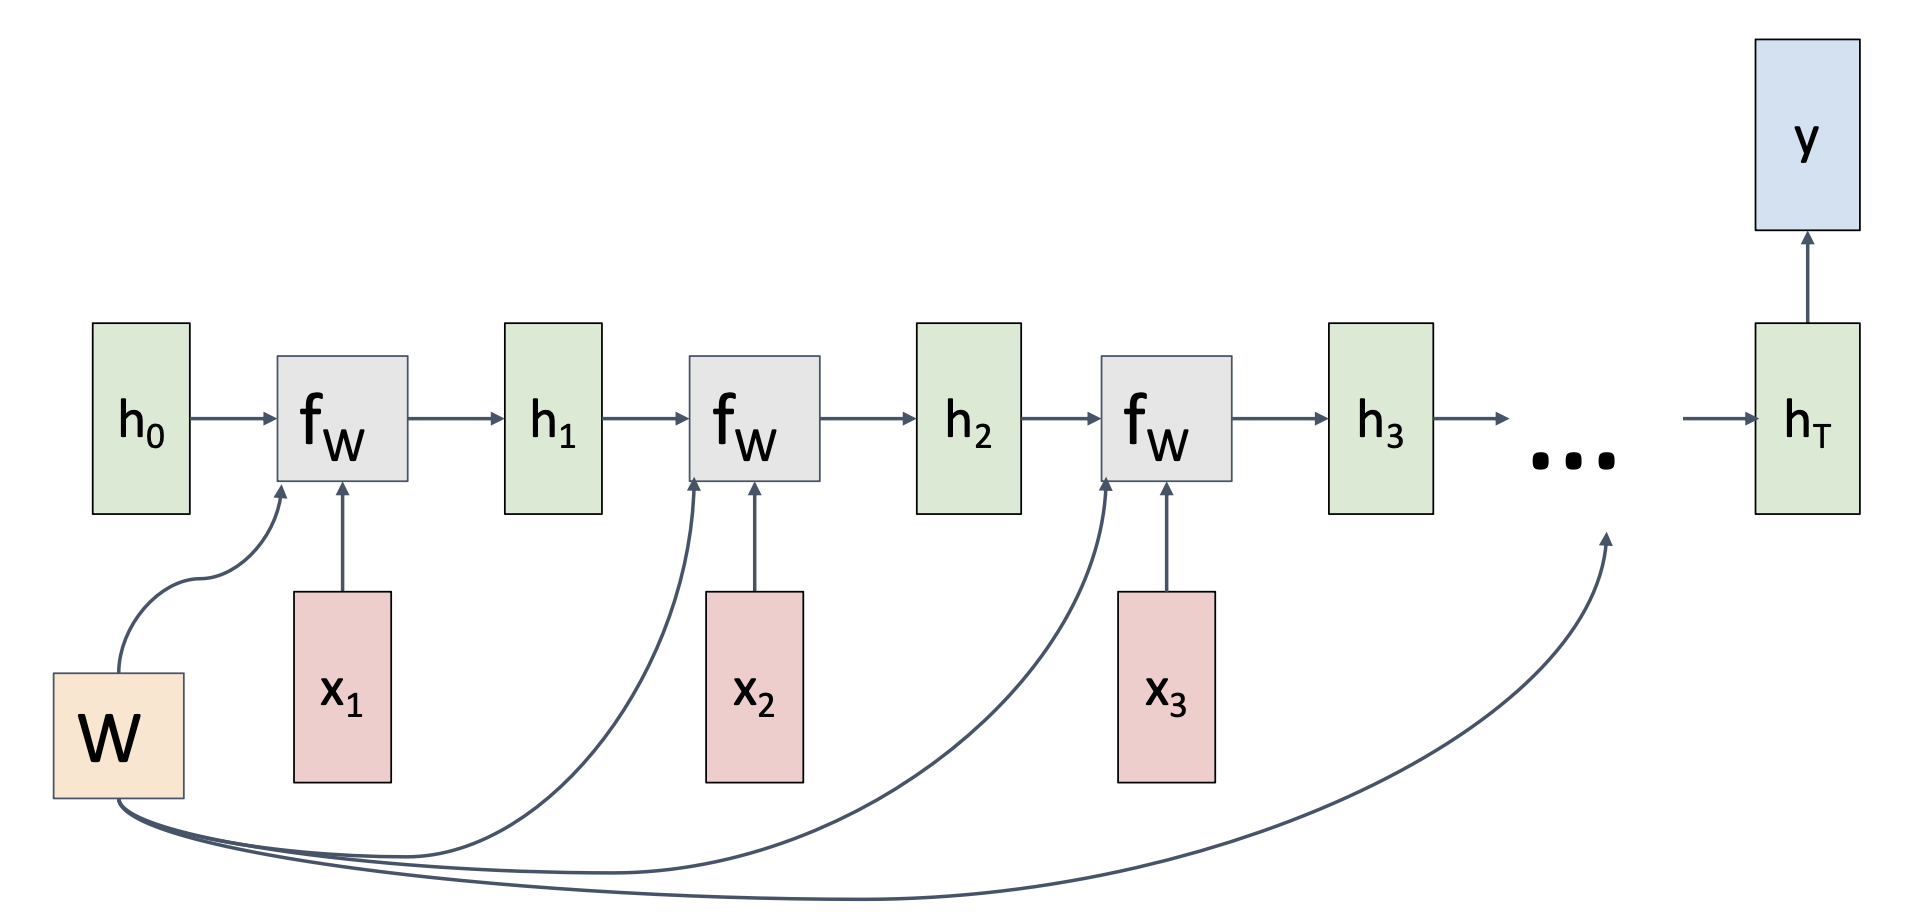
\includegraphics[width=.7\textwidth]{rnn/rnn-many-to-one.png}
    \caption{Many-to-one situation.}
\end{figure}

\paragraph*{One-to-many}
In the one-to-many situation, we typically feed the function with the input only once. After that, the model will keep producing outputs depending solely on the previous hidden state. This generation process usually stops when a certain output is produced, corresponding to some end-of-file token.
\begin{figure}[H]
    \centering
    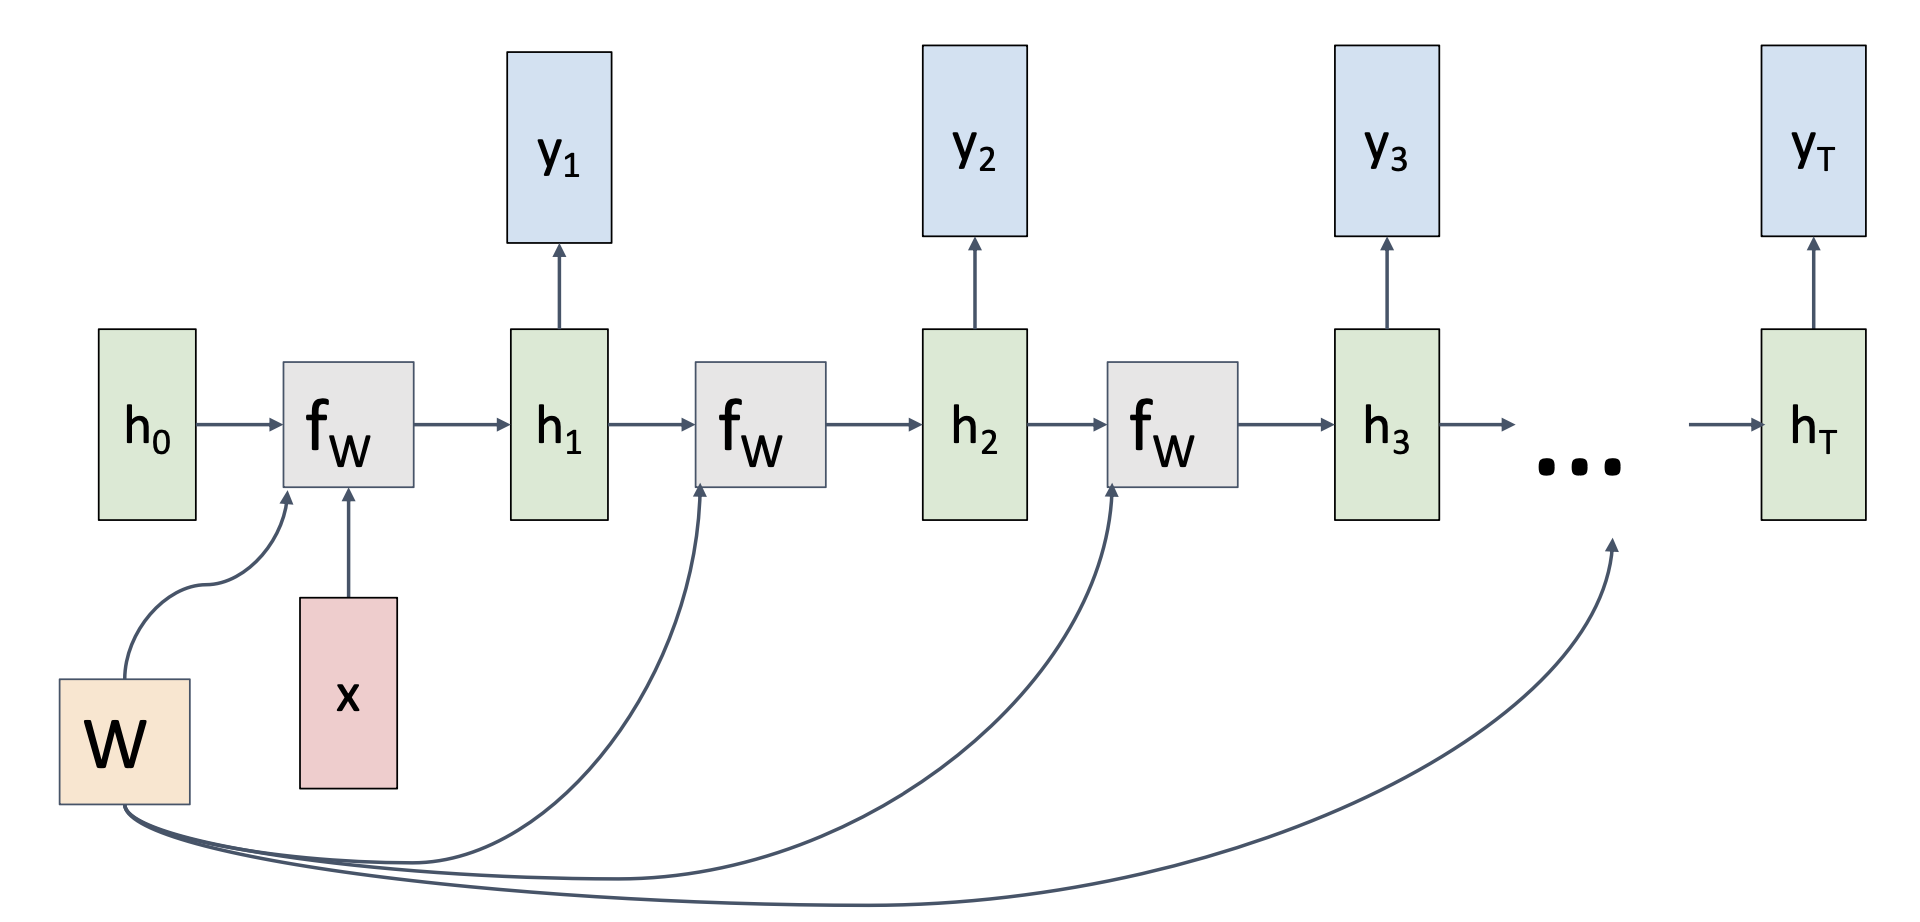
\includegraphics[width=.7\textwidth]{rnn/rnn-one-to-many.png}
    \caption{One-to-many situation.}
\end{figure}

\paragraph*{Many-to-many}
While many-to-one and one-to-many situations are pretty straightforward, many-to-many requires more work, as it would be tricky to manage to make it work with only one recurrent neural network. For instance, in the case of machine translation, it is difficult to produce a translation before the whole input sentence is finished. It seems to be simpler to first read the original sentence, then generate a translated sentence. Furthermore, there is no guarantee that the best hidden states for input understanding are the same as the best hidden states for output generation. Therefore, the sequence to sequence situation is usually handled with two RNNs: an encoder and a decoder.
\begin{figure}[H]
    \centering
    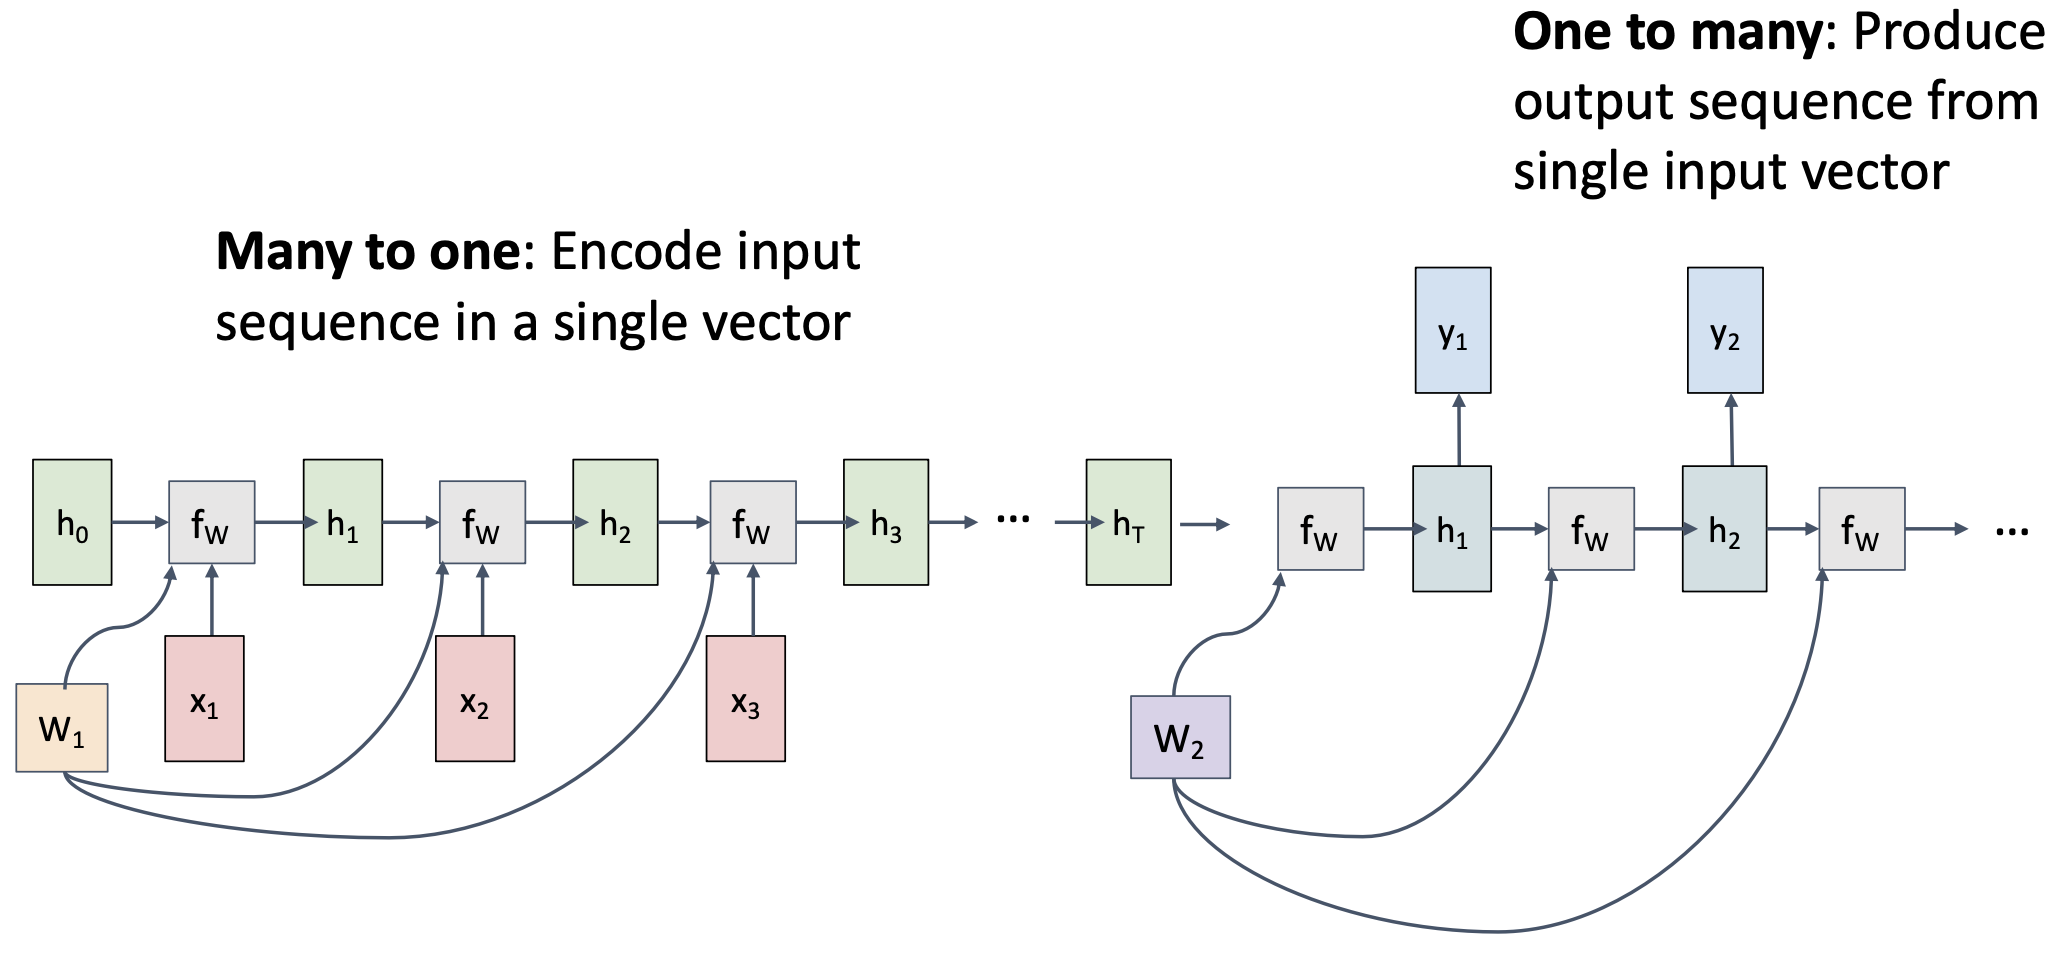
\includegraphics[width=.8\textwidth]{rnn/rnn-many-to-many.png}
    \caption{Encoder and decoder for the many-to-many situation.}
\end{figure}
The encoder will receive the input and summarize it all into the final hidden state of this first many-to-one RNN. This final vector is used by the decoder, a one-to-many RNN, which will use the accumulated context to generate outputs.

\subsubsection{Applications}
Recurrent Neural Networks open the door to many useful and fun applications.

For instance, RNNs can be trained on corpuses of text to generate new sentences following the same style. A nice \texttt{NumPy} implementation of such a vanilla RNN by Andrej Karpathy is available \href{https://gist.github.com/karpathy/d4dee566867f8291f086}{here}\footnote{\href{https://gist.github.com/karpathy/d4dee566867f8291f086}{\nolinkurl{https://gist.github.com/karpathy/d4dee566867f8291f086}}}. When trained on large quantity of text such as Wikipedia, Shakespeare's work or the Linux kernel source code, it can produce new sentences following the style of the text corpus.

\subsection{Gradient Flow in RNNs}
Let's consider the previously introduced vanilla RNN. Its recurrence equation is of the form:
\begin{equation*}
    \begin{aligned}
        h_t &= \tanh\left(W_hh_{t-1}+W_xx_t\right)\\
        &= \tanh\left(W\begin{bmatrix}
            h_{t-1}\\
            x_t
        \end{bmatrix}\right)
    \end{aligned}
\end{equation*}
which corresponds to the following diagram:
\begin{figure}[H]
    \centering
    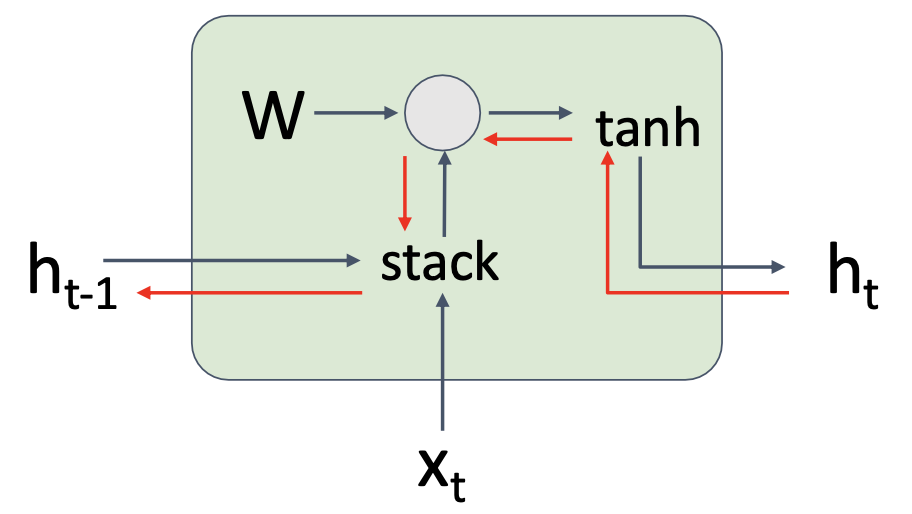
\includegraphics[width=.5\textwidth]{rnn/rnn-backprop.png}
    \caption{Simple computational graph of an RNN cell. Gradient flow is represented in red.}
\end{figure}
This architecture actually causes an issue in the way that the gradient flows throughout the graph. When unrolling the computational graph, we can see that in order to arrive up to $h_0$, the gradient must flow through every previous cell, and will therefore contain as many $W^\tp$ factors as they are time steps.
\begin{figure}[H]
    \centering
    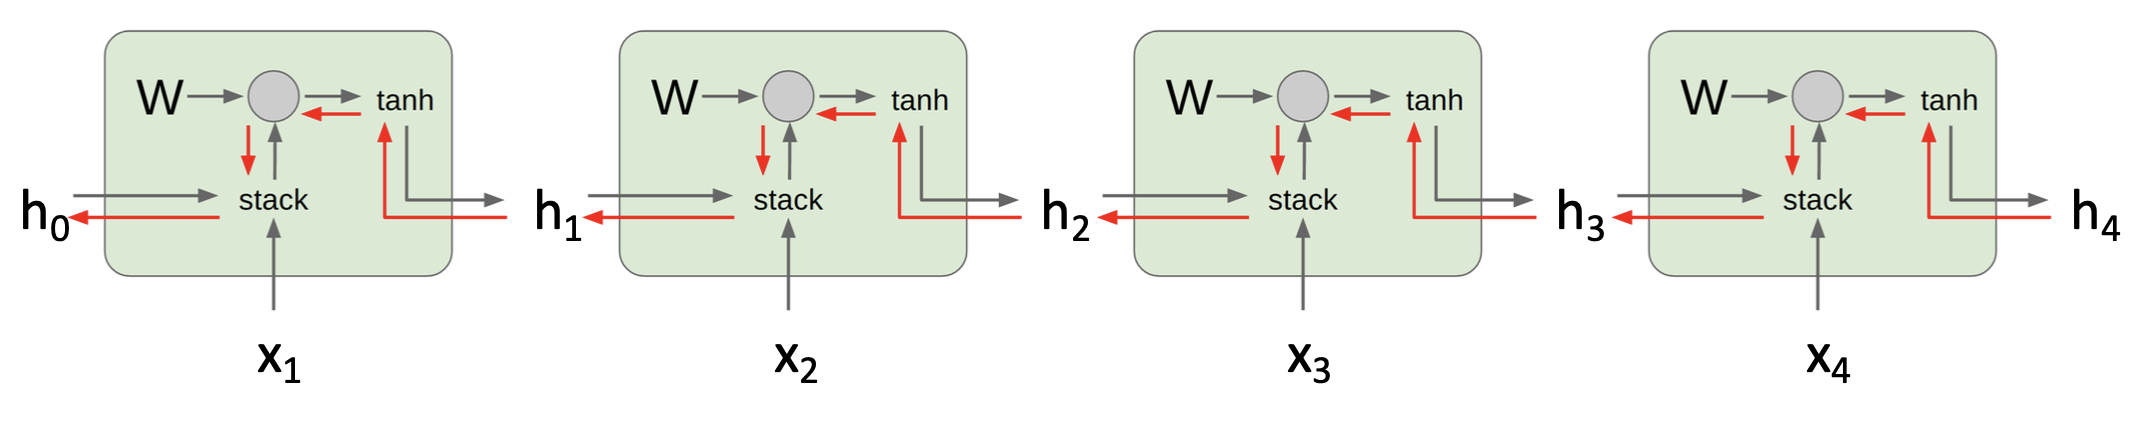
\includegraphics[width=\textwidth]{rnn/rnn-flow-unroll.png}
    \caption{Unrolled computational graph of an RNN. Gradient flow is represented in red.}
\end{figure}
This can cause an issue in one of two possible ways. If the largest eigenvalue of the $W$ matrix is greater than 1, the gradient will explode. If the largest eigenvalue if smaller than 1, the gradient will vanish.

A first solution to avoid the exploding gradient problem is \emph{gradient clipping}. The idea is to scale the gradient if its norm is too big. Formally, we apply the transformation:
\begin{equation*}
    \nabla\L \longleftarrow \begin{cases*}
        \nabla\L \cdot \frac{\theta}{\norm{\nabla\L}} & if $\norm{\nabla\L} > \theta$\\
        \nabla\L & otherwise
    \end{cases*}
\end{equation*}
where $\theta$ is some threshold.

To avoid vanishing gradient, the most widely used solution is to change the recurrent neural network architecture.

\subsection{Long Short-Term Memory (LSTM)}
\subsubsection{Recurrent equation}
The equation defining vanilla recurrent neural network is the following:
\begin{equation}
    h_t = \tanh\left(W\begin{bmatrix}
            h_{t-1}\\
            x_t
        \end{bmatrix}\right)
\end{equation}
The \emph{Long Short-Term Memory} (LSTM) architecture was introduced to solve the vanishing gradient problem. Its recurring equation goes as follows:
\begin{equation*}
    \tag{LSTM}
    \begin{aligned}
        \begin{bmatrix}
            i\\
            f\\
            o\\
            g
        \end{bmatrix}
        &= \begin{bmatrix}
            \sigma\\
            \sigma\\
            \sigma\\
            \tanh
        \end{bmatrix} W \begin{bmatrix}
            h_{t-1}\\
            x_t
        \end{bmatrix} \\
        c_t &= f \odot c_{t-1} + i\odot g\\
        h_t &= o \odot \tanh(c_t)
    \end{aligned}
\end{equation*}
where $\odot$ denotes the Hadamard (component-wise) product.

Instead of keeping only one vector at each time step, two are used: the cell state $c_t$ and the hidden state $h_t$. On top of this, four gates values, $i,f,o$ and $g$ are computed at each time step, which will be used to compute $c_t$ and $h_t$. Each gate can somehow be intuitively interpreted:
\begin{itemize}
    \item \textbf{Input gate} $i$ specifies whether to write in the cell
    \item \textbf{Forget gate} $f$ specifies whether to erase the cell from its previous content
    \item \textbf{Output gate} $o$ specifies how much should the cell be revealed to the hidden state
    \item \textbf{Cell input gate} $g$ specifies what to write in the cell
\end{itemize}
Note that the $g$ gate is the only one to go through a $\tanh$ linearity. The $i,f$ and $o$ gates have coefficients in $[0,1]$, which fits the opened/closed gate interpretation, while $g$ has coefficients in $[-1,1]$, which is the range of values of $c_t$.

The new cell value is a combination of its previous value $c_{t-1}$ and the cell input gate $g$: the proportion of both values are controlled by the forget gate $f$ and the input gate $i$. The new $c_t$ value being computed, it is sent to the classical hidden state $h_t$; the output gate $o$ controls what coefficients are being sent.

\subsubsection{Gradient flow}
While it might seem very complex, LSTM improves the gradient flow throughout the cell. An important behavior is that the gradient propagation from $c_t$ to $c_{t-1}$ only passes through an element-wise multiplication by $f$, and no matrix multiplication by $W^\tp$.
\begin{figure}[H]
    \centering
    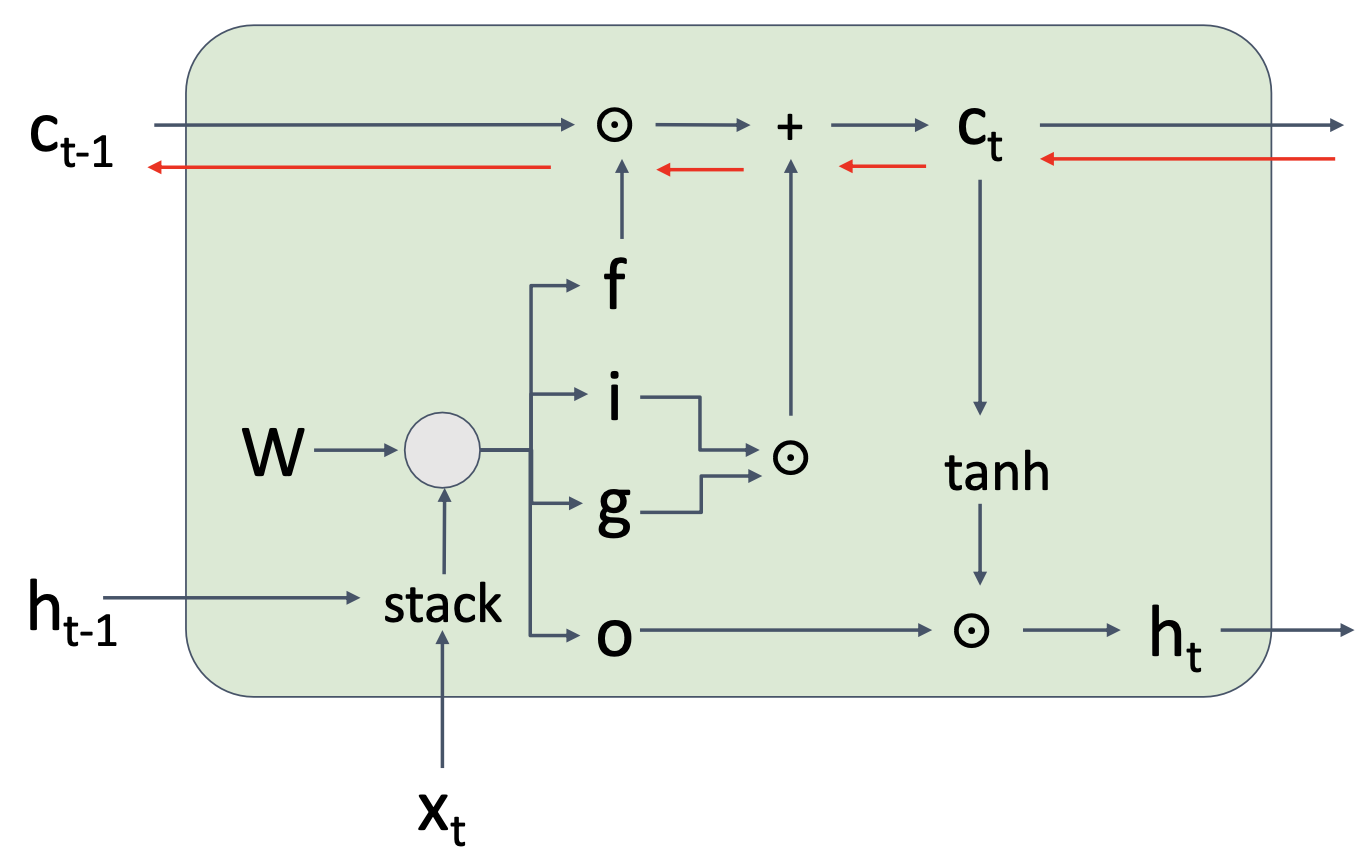
\includegraphics[width=.5\textwidth]{rnn/lstm-flow.png}
    \caption{Gradient flow through an LSTM cell.}
\end{figure}

Therefore, chaining together multiple LSTM cells by unrolling the computational graph does not make the gradient vanish if $f$ is working correctly: it creates an uninterrupted gradient flow from late cell states to early state cells.
\begin{figure}[H]
    \centering
    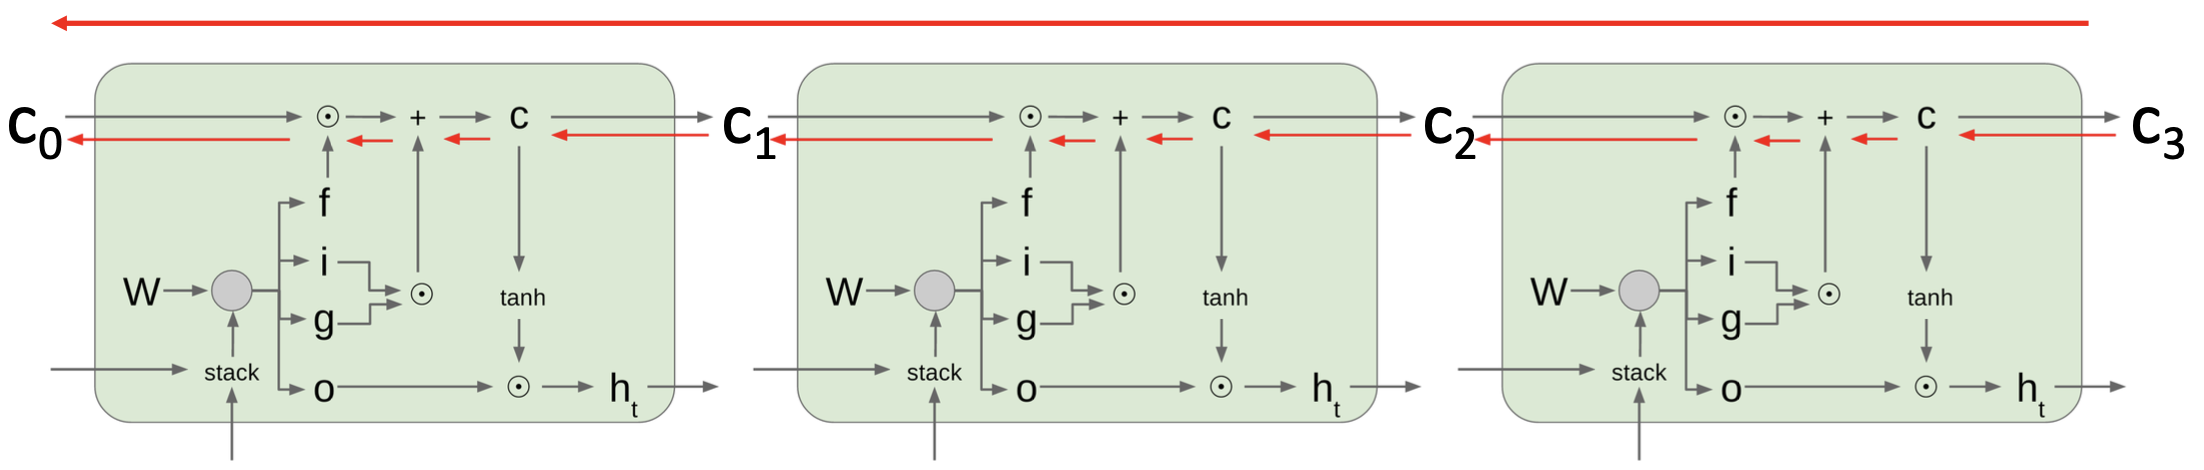
\includegraphics[width=\textwidth]{rnn/lstm-uninterrupted-grad.png}
    \caption{Uninterrupted gradient flow.}
\end{figure}

\subsection{Multilayer Recurrent Neural Networks}
So far, we only considered the use of a recurrent neural network with only one hidden cell. Empirically, neural networks with more layers often perform better, as we saw for MLPs and CNNs. We would like to apply this layering idea to RNNs.

The idea of multilayer RNNs is to feed then hidden states produced at each time steps into a second RNN, with different weight matrices.
\begin{figure}[H]
    \centering
    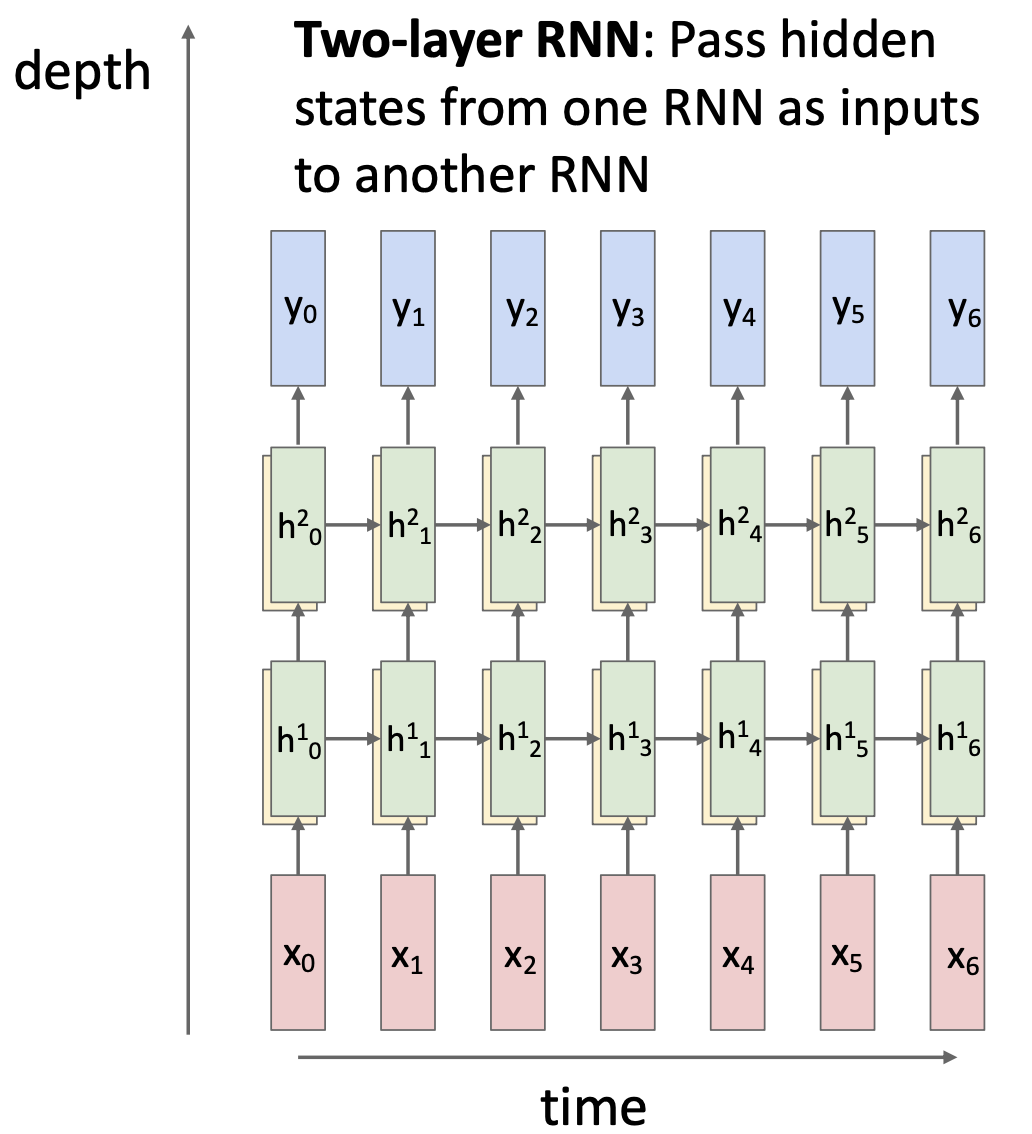
\includegraphics[width=.5\textwidth]{rnn/two-layer-rnn.png}
    \caption{A two-layer RNN.}
\end{figure}
This process can be iterated to create deep recurrent neural networks, by adding two, three, ore more RNNs on top of each other. Note that while it is very common for CNNs to have very deep networks, RNNs are often used in practice with no more than three or four layers.

\subsection*{RNN: Summary}
RNNs give us a lot of flexibility in architecture design by allowing one/many to one/many models. Vanilla RNNs are simple but don't work so well, because of exploding and vanishing gradients. LSTM is the most commonly used alternative to vanilla RNNs, used to solve the vanishing gradient problem.

%But RNNs cells can also be combined to form multi-layer architectures. In a multi-layer RNN, the input is fed into a first hidden state, which is then used as the input for a second hidden state (another layer), which is eventually passed into a feed-forward layer to produce an output.